\subsection{Shannon-Nyquist-Abtasttheorem} % (fold)
\label{sub:Shannon-Nyquist-Abtasttheorem}

\begin{frame}
    \frametitle{Erhöhung der Frequenz}
    \framesubtitle{}
     \begin{block}{}
         \begin{itemize}
             \item Zunächst wird der Tiefpassfilter überbrückt
             \item Erhöhung der Frequenz mit allen Bits gesetzt
         \end{itemize}
     \end{block}
\end{frame}
\begin{frame}
    \frametitle{Erhöhung der Frequenz}
    \framesubtitle{100Hz}
            \begin{figure}[H]
            \begin{center}
                    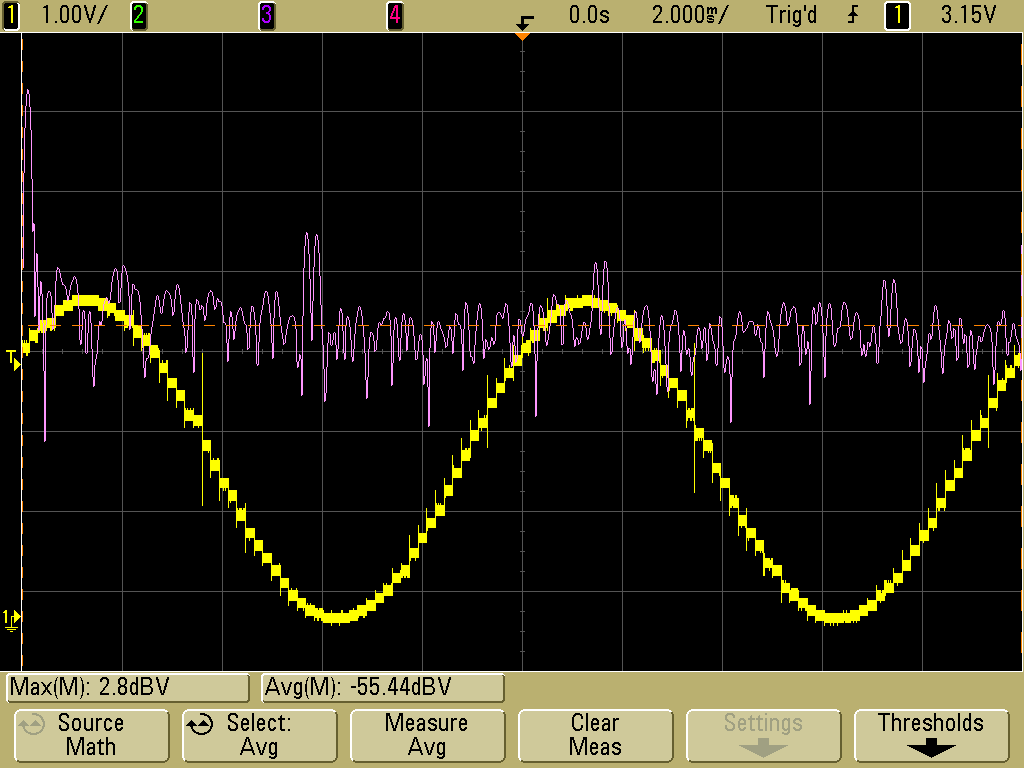
\includegraphics[scale=0.2]{./img/oszi/scope_21.png}
            \end{center}
            \end{figure}
\end{frame}
\begin{frame}
    \frametitle{Erhöhung der Frequenz}
    \framesubtitle{500Hz}
            \begin{figure}[H]
            \begin{center}
                    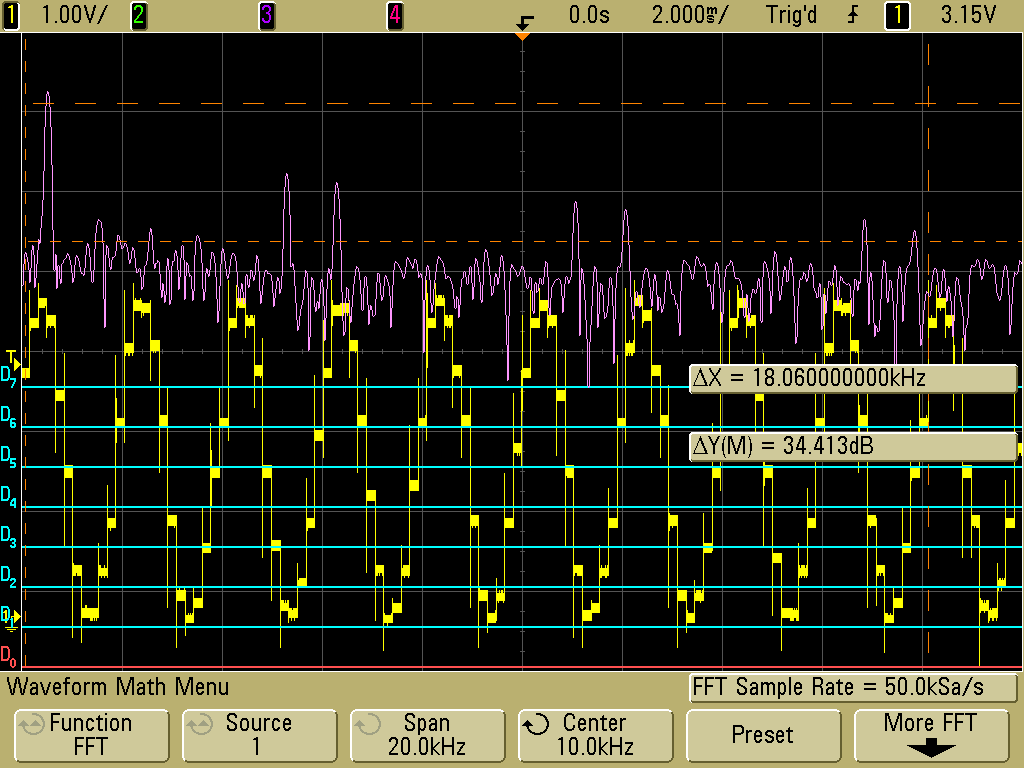
\includegraphics[scale=0.2]{./img/oszi/scope_20.png}
            \end{center}
            \end{figure}
\end{frame}
\begin{frame}
    \frametitle{Erhöhung der Frequenz}
    \framesubtitle{800Hz}
            \begin{figure}[H]
            \begin{center}
                    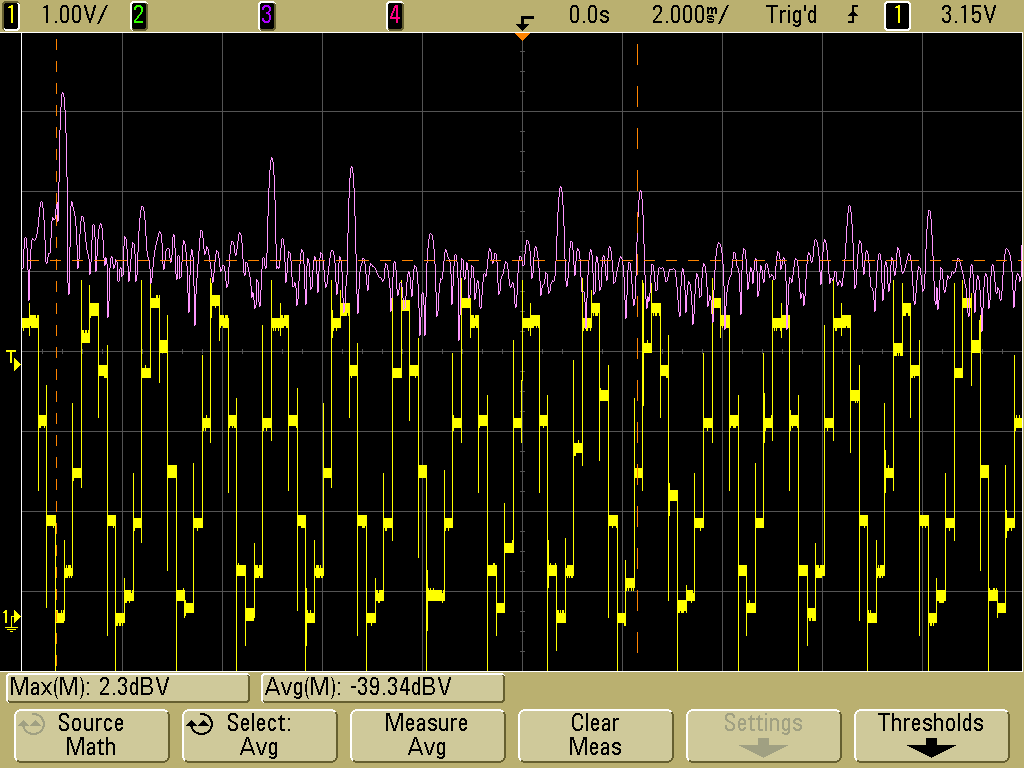
\includegraphics[scale=0.2]{./img/oszi/scope_22.png}
            \end{center}
            \end{figure}
\end{frame}
\begin{frame}
    \frametitle{Erhöhung der Frequenz}
    \framesubtitle{1500Hz}
            \begin{figure}[H]
            \begin{center}
                    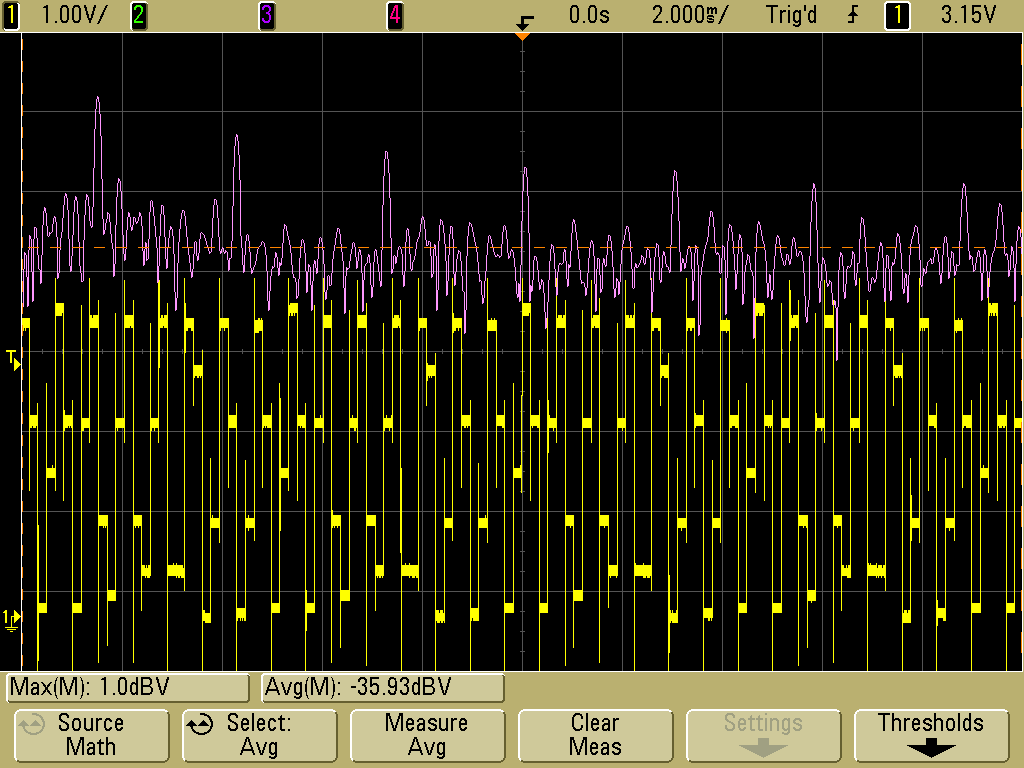
\includegraphics[scale=0.2]{./img/oszi/scope_23.png}
            \end{center}
            \end{figure}
\end{frame}
\begin{frame}
    \frametitle{Erhöhung der Frequenz}
    \framesubtitle{2300Hz}
            \begin{figure}[H]
            \begin{center}
                    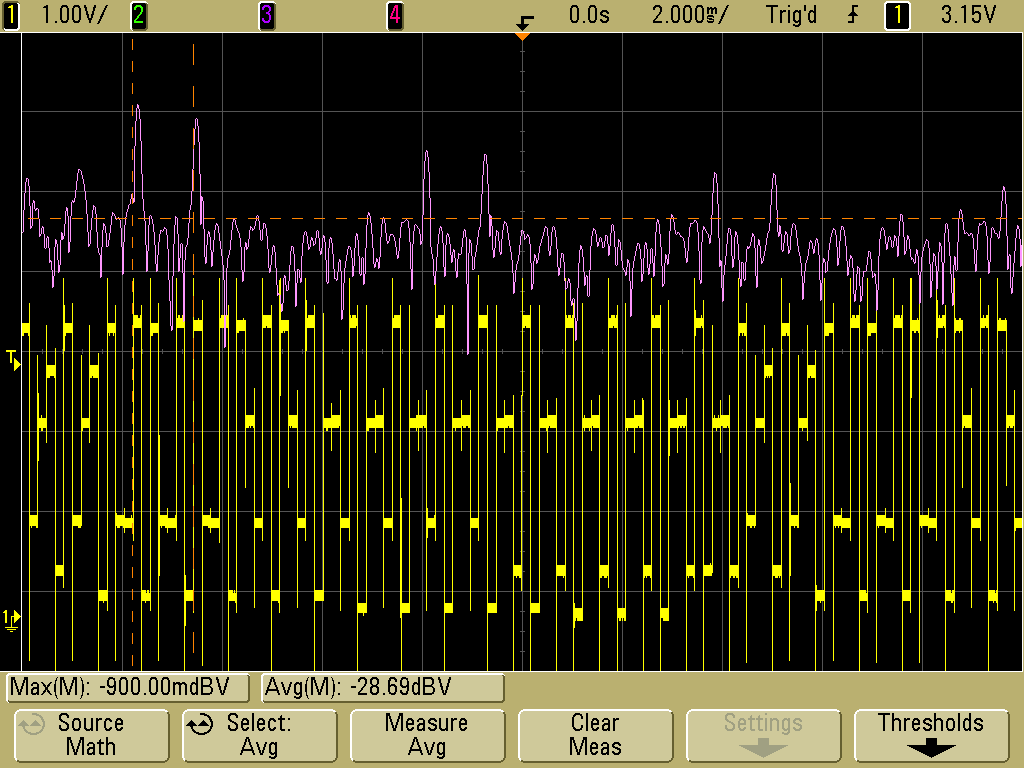
\includegraphics[scale=0.2]{./img/oszi/scope_24.png}
            \end{center}
            \end{figure}
\end{frame}
\begin{frame}
    \frametitle{Erhöhung der Frequenz}
    \framesubtitle{2700Hz}
            \begin{figure}[H]
            \begin{center}
                    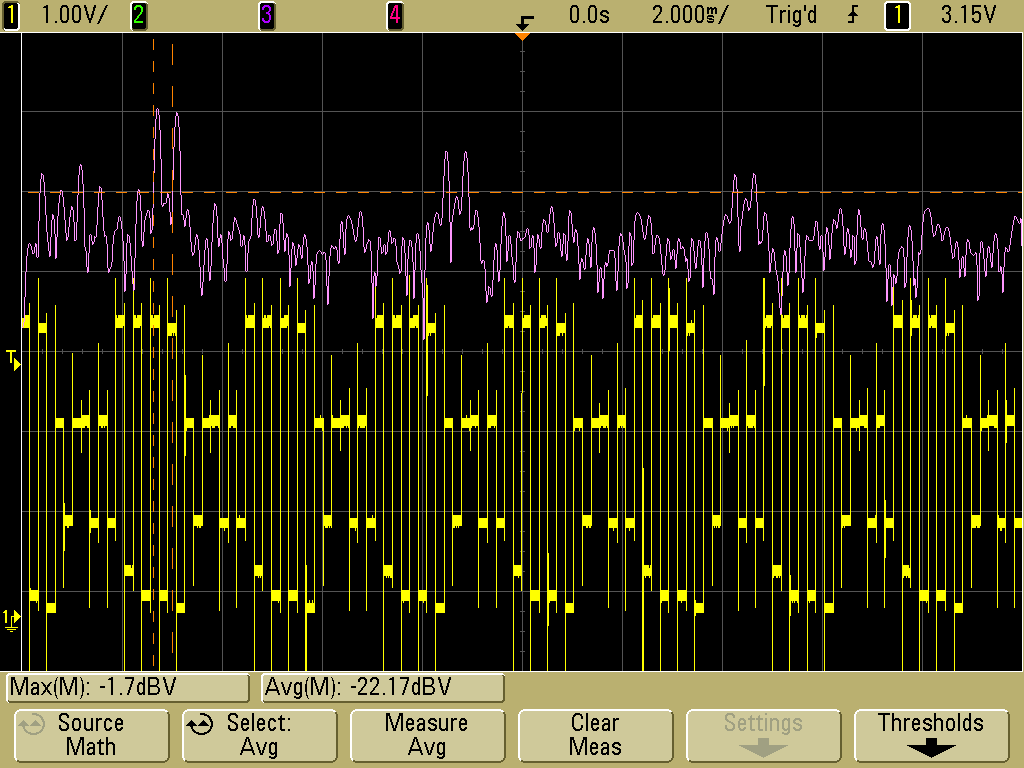
\includegraphics[scale=0.2]{./img/oszi/scope_25.png}
            \end{center}
            \end{figure}
\end{frame}
\begin{frame}
    \frametitle{Erhöhung der Frequenz}
    \framesubtitle{2900Hz}
            \begin{figure}[H]
            \begin{center}
                    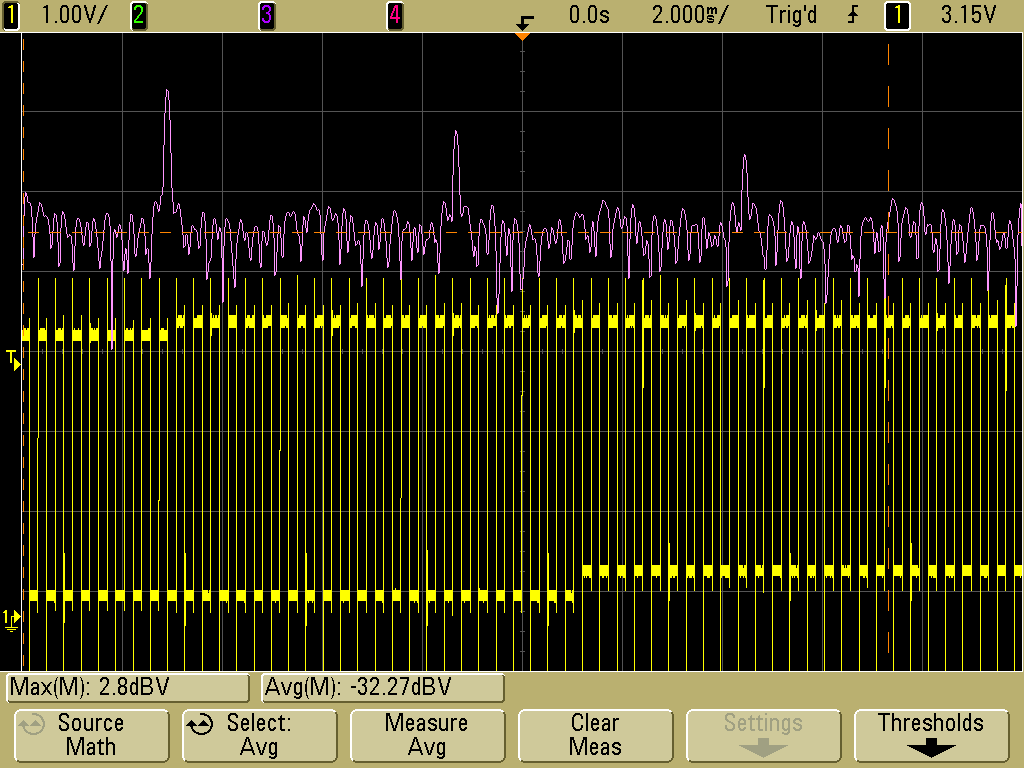
\includegraphics[scale=0.2]{./img/oszi/scope_26.png}
            \end{center}
            \end{figure}
\end{frame}
\begin{frame}
    \frametitle{Erhöhung der Frequenz}
    \framesubtitle{3500Hz}
            \begin{figure}[H]
            \begin{center}
                    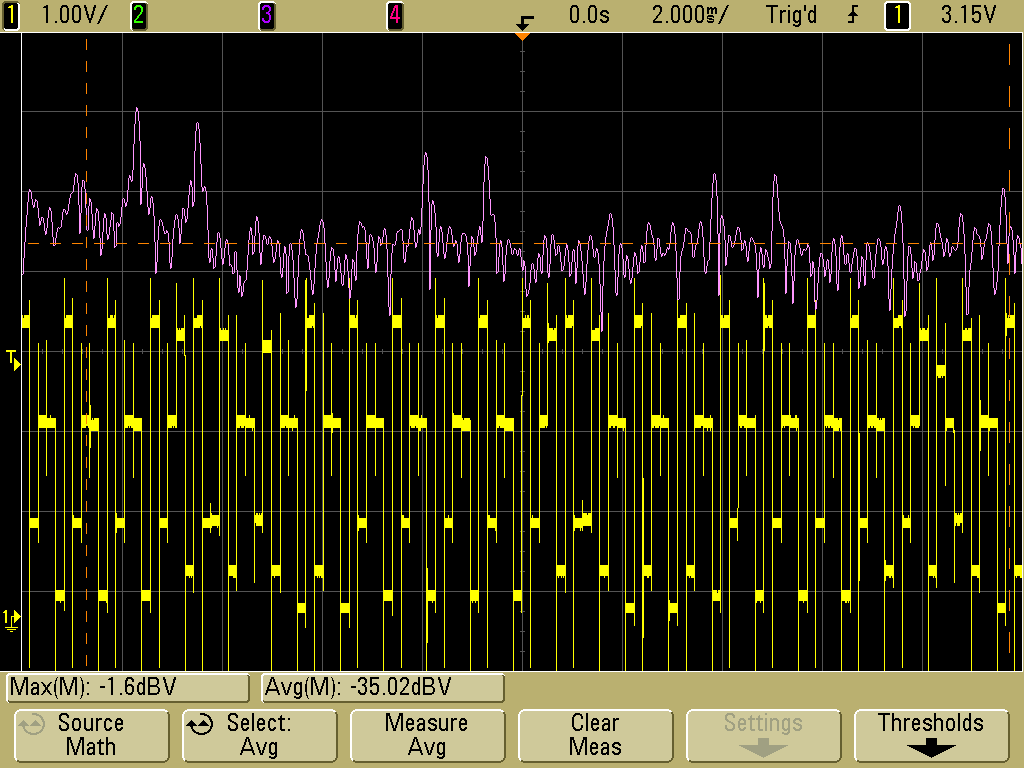
\includegraphics[scale=0.2]{./img/oszi/scope_27.png}
            \end{center}
            \end{figure}
\end{frame}
\begin{frame}
    \frametitle{Erhöhung der Frequenz}
    \framesubtitle{5000Hz}
            \begin{figure}[H]
            \begin{center}
                    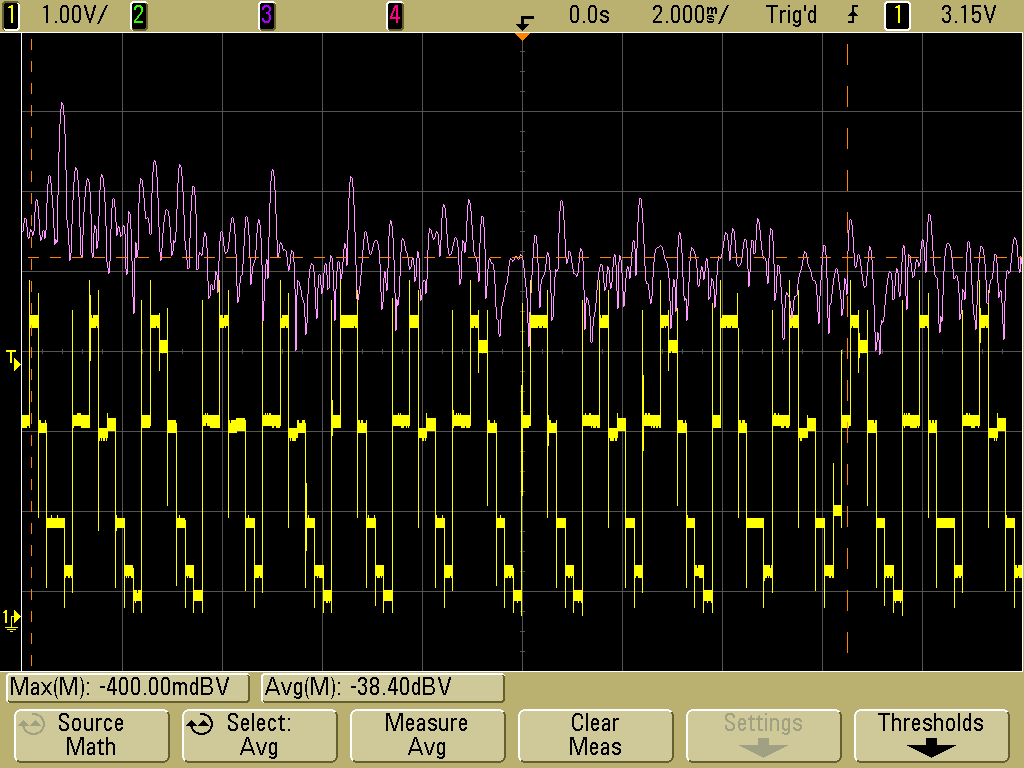
\includegraphics[scale=0.2]{./img/oszi/scope_28.png}
            \end{center}
            \end{figure}
\end{frame}
\begin{frame}
    \frametitle{Erhöhung der Frequenz}
    \framesubtitle{18000Hz}
            \begin{figure}[H]
            \begin{center}
                    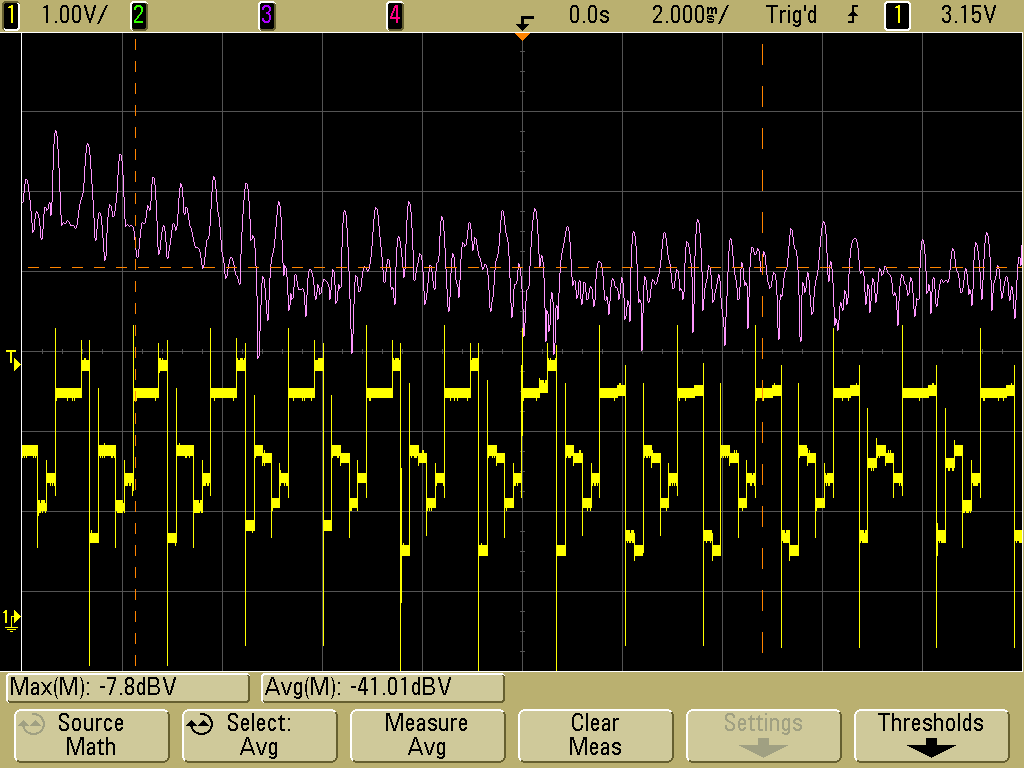
\includegraphics[scale=0.2]{./img/oszi/scope_29.png}
            \end{center}
            \end{figure}
\end{frame}
\begin{frame}
    \frametitle{Beobachtungen}
    \framesubtitle{}
    \begin{block}{Signalentwicklung}
        \begin{itemize}
            \item Je höher die Signalfrequenz, desto weniger Zeit bleibt einen
            Wellenberg abzutasten (Signal wird "eckiger")
            \item liegt Signalfrequenz nah an Abtastfrequenz enstehen
            Schwebungseffekte
            \item sehr hohe Spannung verzerren das Signal, aber Periodizität
            bleibt
        \end{itemize}
    \end{block}
    \begin{block}{Frequenzentwicklung}
        \begin{itemize}
            \item je mehr das digitalisierte Signal vom Sinus abweicht desto
            mehr Peaks enstehen durch die Furrieranalyse
            \item gegenläufige Frequenzpeaks $\rightarrow$ oszillierender Ton
        \end{itemize}
    \end{block}
\end{frame}
\begin{frame}
    \frametitle{Einbauf von Tiefpassfilter}
    \framesubtitle{}
    \begin{block}{}
        Nun wird der Tiefpassfilter eingebaut
    \end{block}
    \begin{figure}[H]
    \begin{center}
            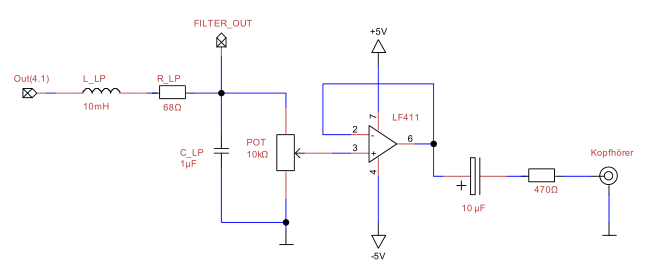
\includegraphics[scale=0.5]{./img/schaltung/verstaerker.png}
    \end{center}
    \end{figure}
\end{frame}

\begin{frame}
    \frametitle{Tiefpassfilter I}
    \framesubtitle{100Hz}
    \begin{figure}[H]
    \begin{center}
            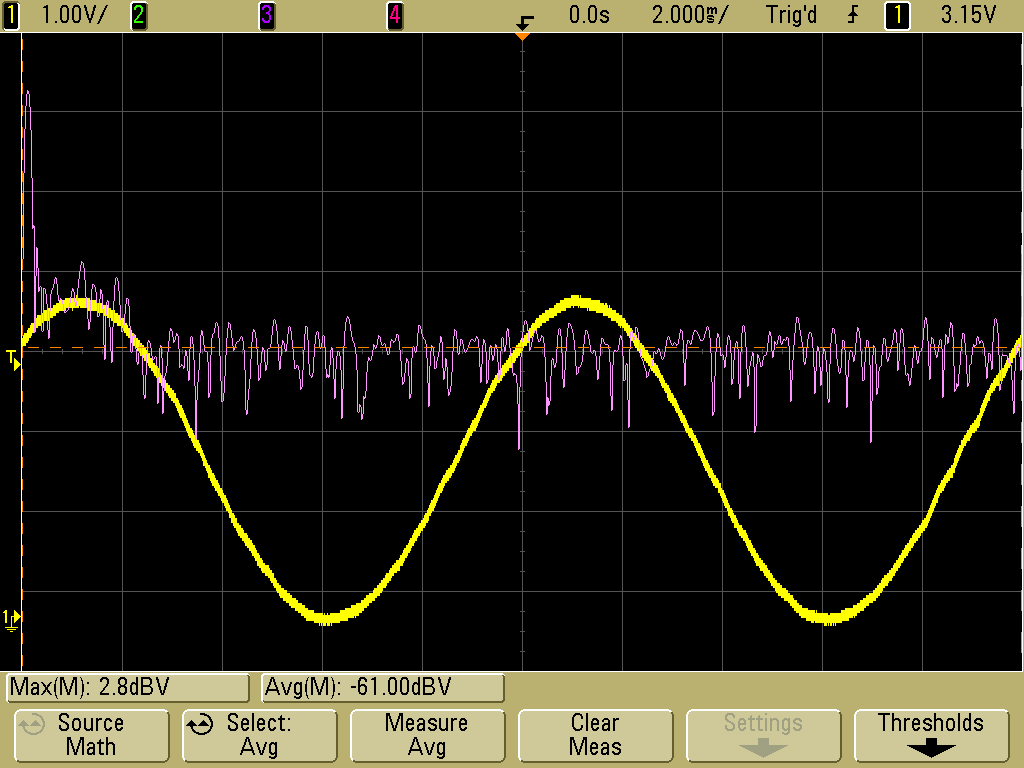
\includegraphics[scale=0.15]{./img/oszi/scope_30.png}
    \end{center}
    \end{figure}  
\end{frame}
\begin{frame}
    \frametitle{Tiefpassfilter I}
    \framesubtitle{700Hz}
    \begin{figure}[H]
    \begin{center}
            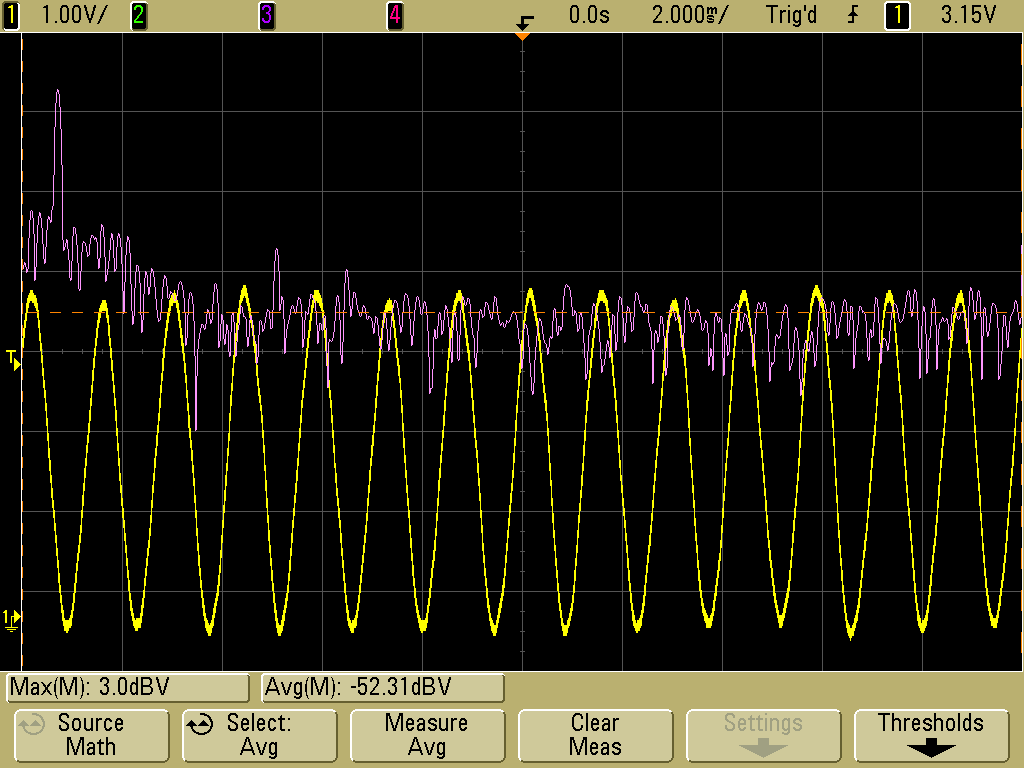
\includegraphics[scale=0.15]{./img/oszi/scope_31.png}
    \end{center}
    \end{figure}  
\end{frame}
\begin{frame}
    \frametitle{Tiefpassfilter I}
    \framesubtitle{1500Hz}
    \begin{figure}[H]
    \begin{center}
            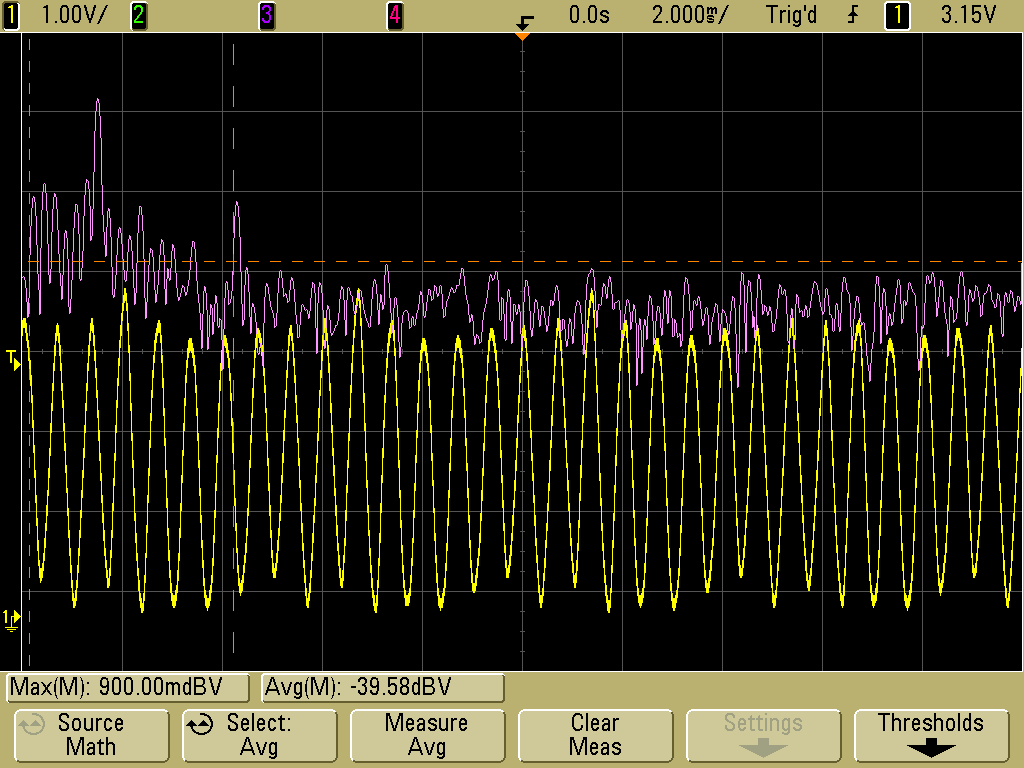
\includegraphics[scale=0.15]{./img/oszi/scope_32.png}
    \end{center}
    \end{figure}  
\end{frame}
\begin{frame}
    \frametitle{Tiefpassfilter I}
    \framesubtitle{2800Hz}
    \begin{figure}[H]
    \begin{center}
            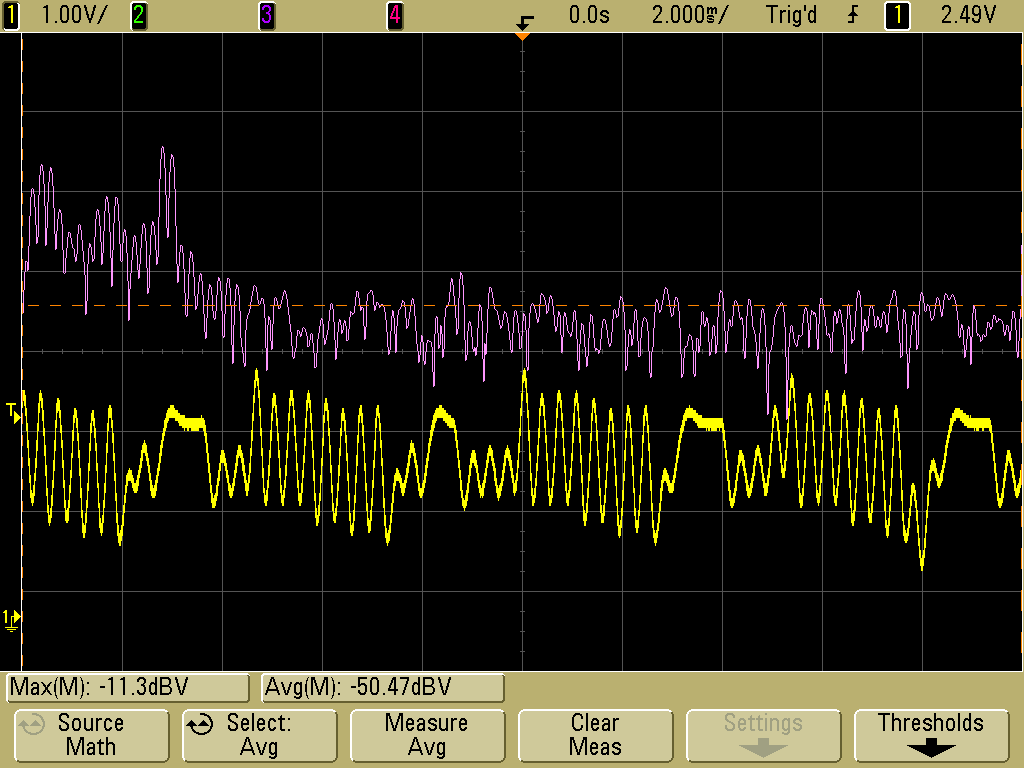
\includegraphics[scale=0.15]{./img/oszi/scope_33.png}
    \end{center}
    \end{figure}  
\end{frame}
\begin{frame}
    \frametitle{Tiefpassfilter I}
    \framesubtitle{Vergleich 1500Hz}
    \begin{columns}[c]
        \column{0.5\textwidth}
            \begin{figure}[H]
            \begin{center}
                    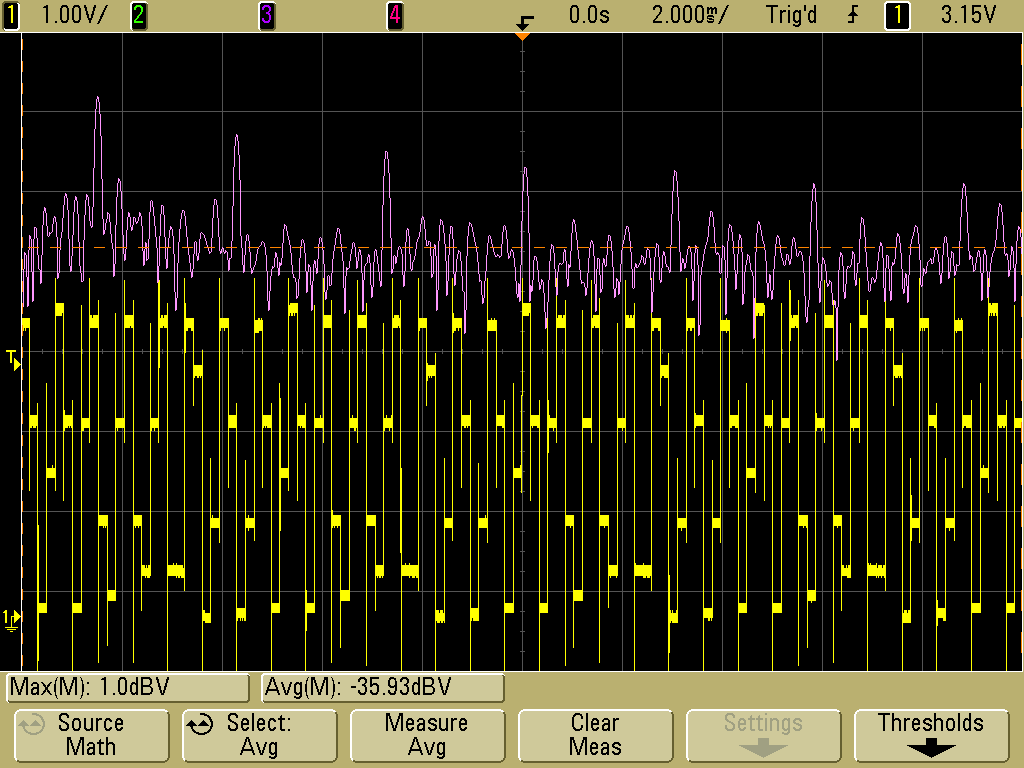
\includegraphics[scale=0.12]{./img/oszi/scope_23.png}
            \end{center}
            \caption{Ohne Tiefpassfilter}
            \end{figure}  
        \column{0.5\textwidth}
            \begin{figure}[H]
            \begin{center}
                    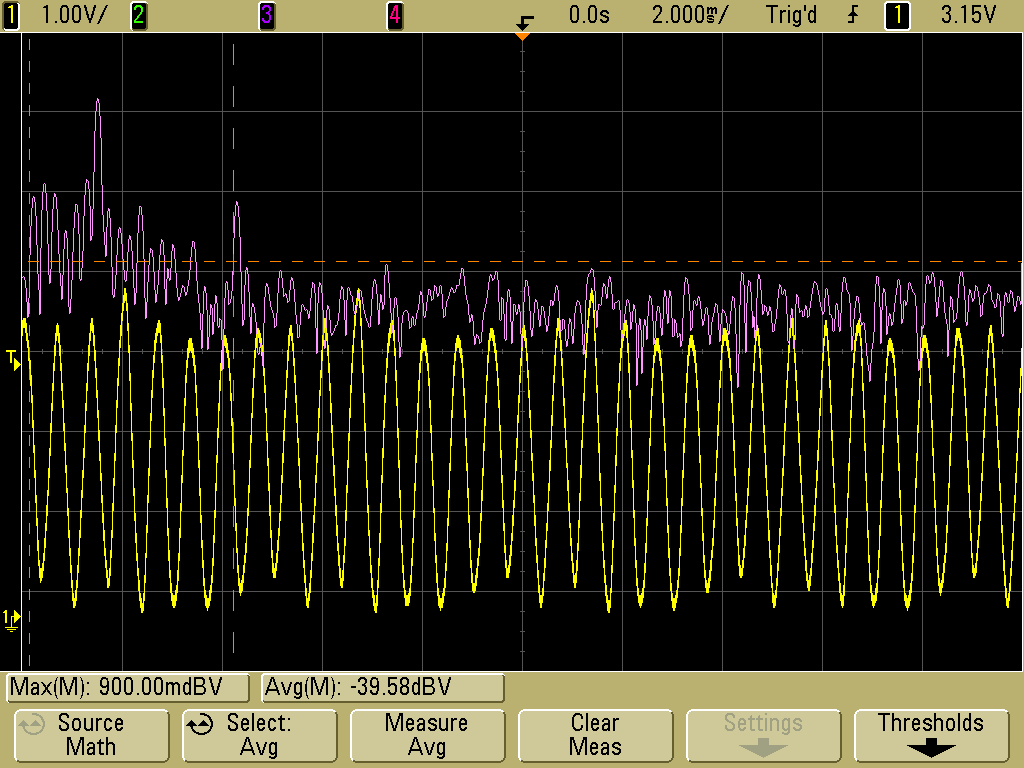
\includegraphics[scale=0.12]{./img/oszi/scope_32.png}
            \end{center}
            \caption{Mit Tiefpassfilter}
            \end{figure}  
    \end{columns}
    \begin{block}{Vergleich}
        \begin{itemize}
            \item Tiefpassfilter filtert ungewünschte hohe Frequenzen heraus
            \item deutlich besseres Signal
            \item schwächeres Gegeneinanderlaufen $\rightarrow$ weniger Ton-Oszillation
        \end{itemize}
    \end{block}
\end{frame}
\begin{frame}
    \frametitle{Tiefpassfilter II}
    \framesubtitle{}
    \begin{block}{Zusätzlicher Tiefpassfilter}
         \begin{itemize}
             \item Zusätzlicher Tiefpassfilter am Eingang des A/D Wandlers 
             \item es wurde keine Veränderung des Signals beobachtet
         \end{itemize}
    \end{block}
\end{frame}

% subsection Shannon-Nyquist-Abtasttheorem (end)
